\chapter{DESENVOLVIMENTO}
\label{cap:desenvolvimento}

Neste capítulo serão apresentados os projetos e tecnologias utilizadas durante o tempo de estágio experienciado.

Na sua grande maioria, os projetos do LEMAF são sistemas web, constituídos de uma aplicação backend e uma frontend.

O backend durante o desenvolvimento muitas vezes é rodado no computador do próprio dev, porem quando há necessidade de serem feitos testes, é criado um servidor dentro da rede local para que possam ser efetuados os mesmo, sendo mais precisos por conta de estarem em um servidor.

A infraestrutura de servidores do lemaf muitas vezes são servidores com diversas maquinas, todas rodando NGNIX para prover as aplicações.

O frontend geralmente seguia o mesmo processo do backend, porem quando ia para alguma maquina externa, era criado alguma configuração para que o backend servisse o frontend, evitando assim problemas de CORS.

Já o banco de dados era controlado por um DBA(Database Administrator), que criava e gerenciava toda a estrutura de banco, sendo somente necessário aos devs, discutir melhores soluções e criar tarefas para os mesmos.

Durante meu 1 ano como estagiário, participei de todos squads, trabalhando com diversos times, projetos e tecnologias.

Em minha primeira equipe(Squad 1 - Carreta Furacão), tive como tecnologias necessárias JAVA(backend) e Angular(Frontend), para que fosse possível evoluir os projetos do Cadastro Ambiental Rural, incluindo os projetos SICAR, Central do Responsavel Tecnico, Central do Proprietario, PRA-OFF.

\begin{figure}[H]
\centering
\caption{SICAR-PA} %legenda
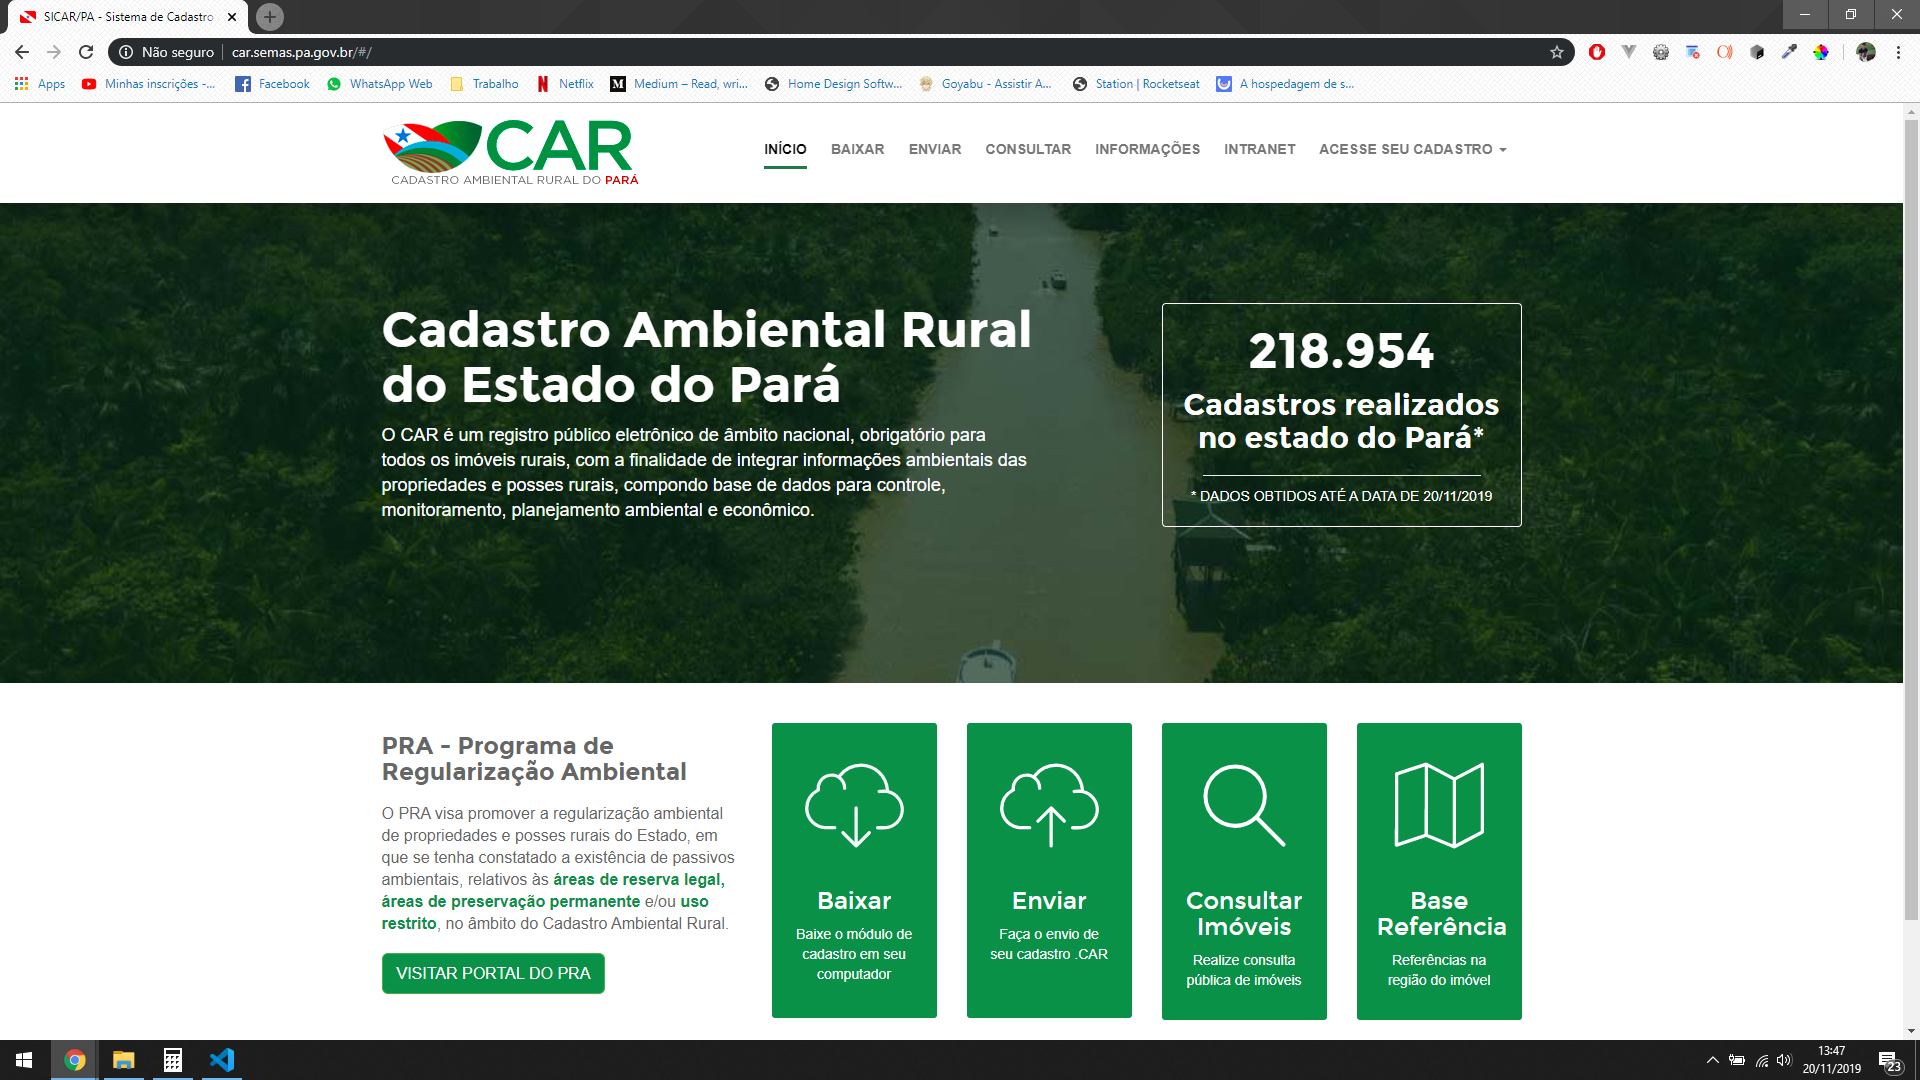
\includegraphics[scale=0.3]{SICAR}\\  % o 0.9 indica 90% do tamanho original
% pdfLaTeX aceita figuras no formato PNG, JPG ou PDF
% figuras vetoriais podem ser exportadas para eps e depois convertidas para pdf usando epstopdf
{\small Fonte: http://car.semas.pa.gov.br/#/} %Fonte da imagem
\label{fig:exemplo} %rotulo para refencia
\end{figure}

O projeto do SICAR tinha como objetivo informar e controlar os cadastros ambientais rurais feitos no estado do pará, sendo necessária algumas integrações com os módulos do SICAR federal e as Centrais ligadas ao PRA.

\begin{figure}[H]
\centering
\caption{PRA-OFF} %legenda
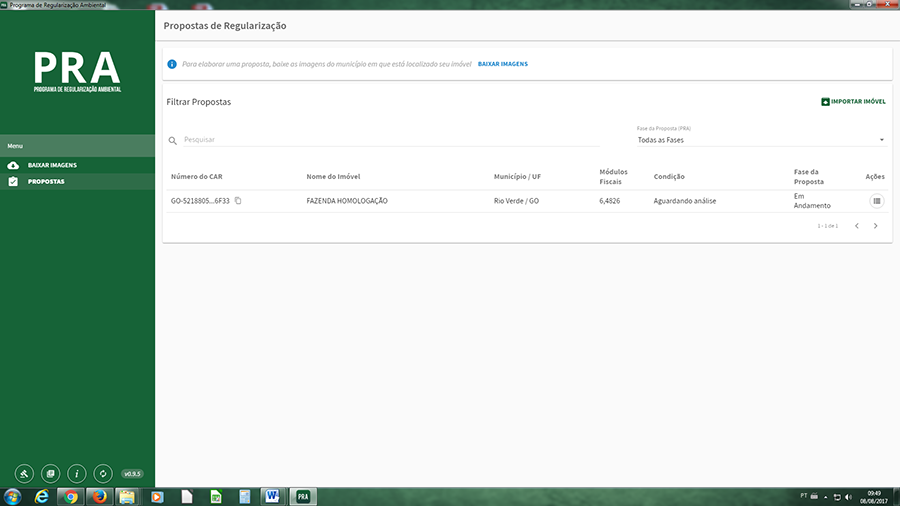
\includegraphics[scale=0.5]{pra-off}\\  % o 0.9 indica 90% do tamanho original
% pdfLaTeX aceita figuras no formato PNG, JPG ou PDF
% figuras vetoriais podem ser exportadas para eps e depois convertidas para pdf usando epstopdf
{\small Fonte: http://www.cprh.pe.gov.br/Controle_Ambiental/Sistema%20Nacional%20de%20Cadastro%20Ambiental%20Rural%20-%20Sicar/PRA/43052%3B53356%3B480802%3B0%3B0.asp} %Fonte da imagem
\label{fig:exemplo} %rotulo para refencia
\end{figure}

Já o projeto do PRA, não era possíveis tais integrações, pois ele era um modulo offline, sendo possível a utilização sem internet. Para o desenvolvimento do mesmo, foi necessário estudar sobre electron, uma ferramenta que possibilita criar modulos web em aplicações offiline.

Após 5 meses a equipe foi quebrada em duas e então foi feita uma redistribuição de projetos e acabei indo para a tribo Runners. Os projetos principais que contribui durante esse período foram o Consulta Publica - PARÁ e relatórios do PRA.

\begin{figure}[H]
\centering
\caption{Consulta publica} %legenda
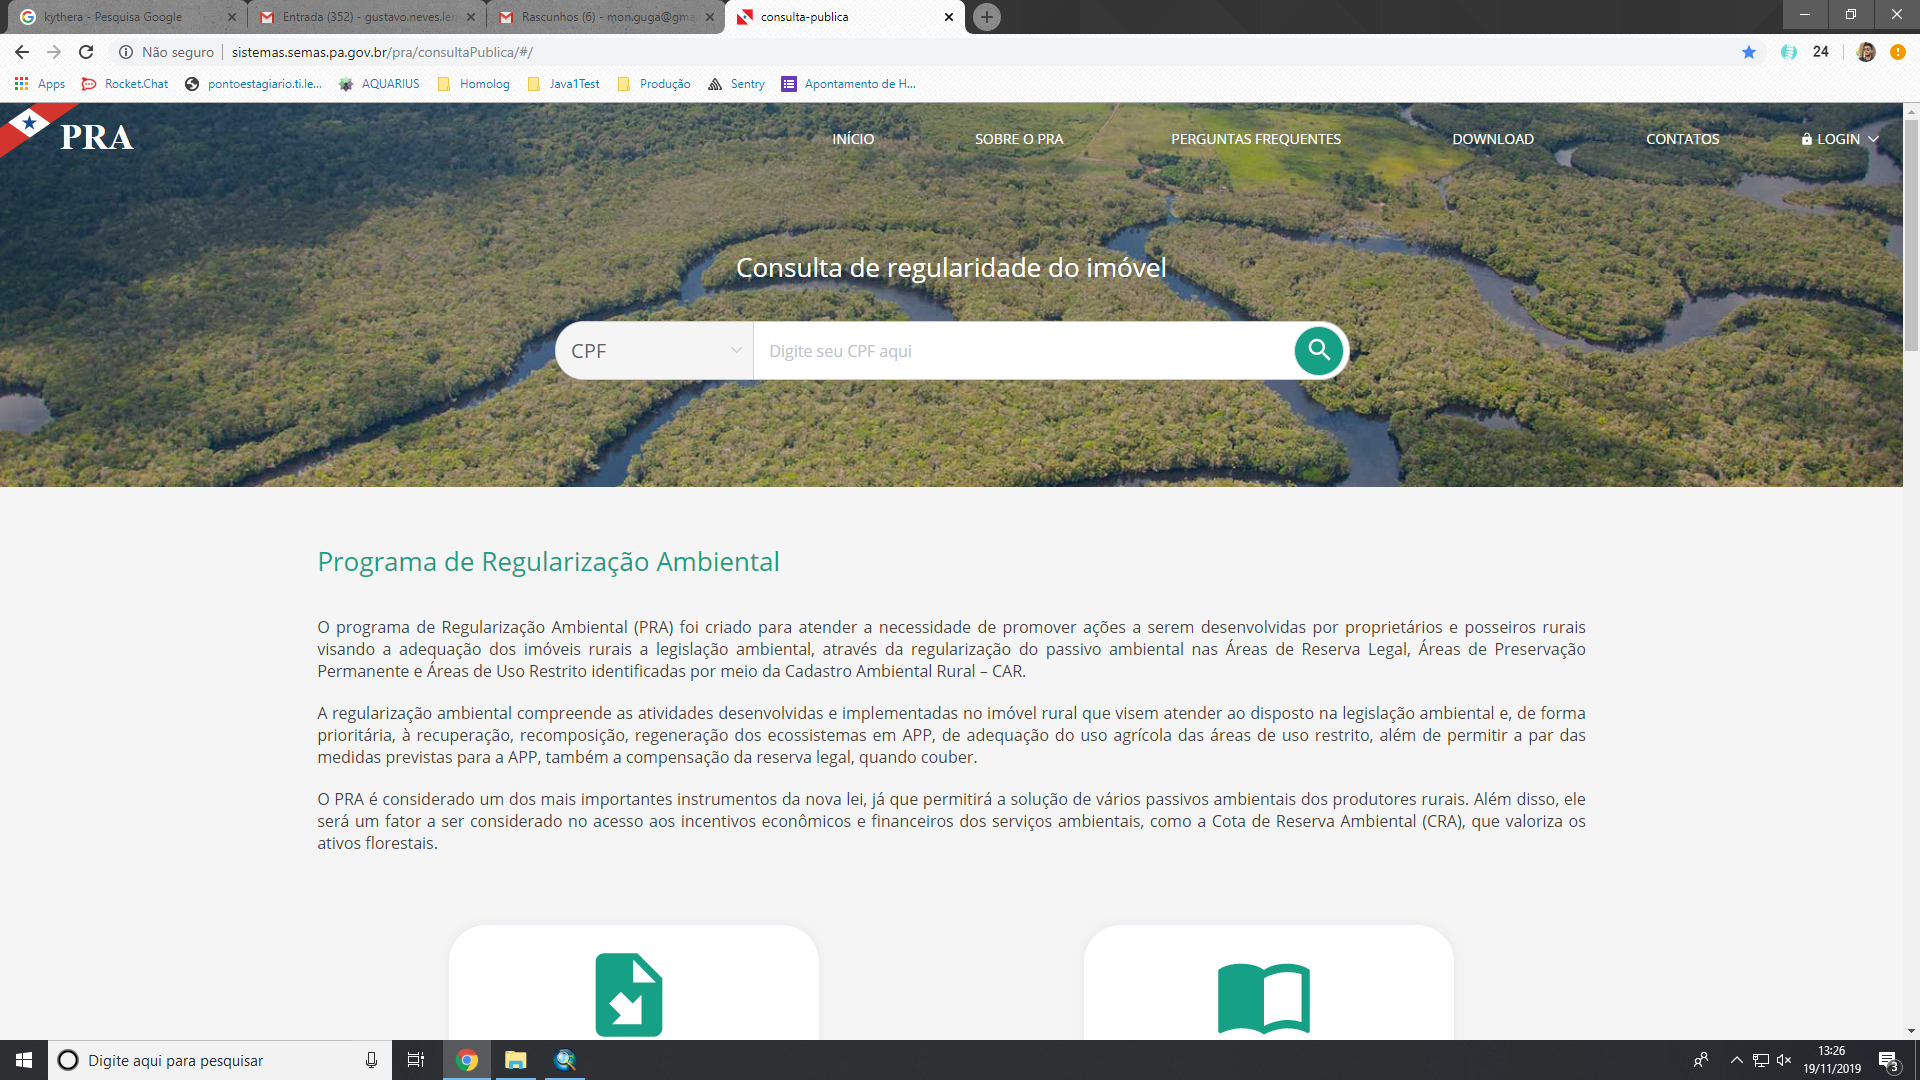
\includegraphics[scale=0.22]{consulta-publica}\\  % o 0.9 indica 90% do tamanho original
% pdfLaTeX aceita figuras no formato PNG, JPG ou PDF
% figuras vetoriais podem ser exportadas para eps e depois convertidas para pdf usando epstopdf
{\small Fonte: http://sistemas.semas.pa.gov.br/pra/consultaPublica/#/} %Fonte da imagem
\label{fig:exemplo} %rotulo para refencia
\end{figure}

O projeto consulta publica foi o primeiro projeto que tive como objetivo a refatoração, pois o projeto era antigo, utilizava uma das primeiras versões de VueJs no frontend e tinha o layout bem ruim.
Foi a primeira obrigação que tive total responsabilidade, tinha que migrar todo o sistema para VueJs 2.0 e refatorar o frontend.

Como era minha primeira experiencia com o framework VueJs, o projeto foi bem demorado, tive suporte do meu time que me tutoreava sobre arquitetura, padrões de projetos, boas praticas.
Para melhor aprendizado meu e um controle sobre códigos ruins, todas modificações feitas por mim sempre passavam por um Code Review e só quando aprovadas, eram enviadas para o projeto. 

O projeto consulta publica tinha como objetivo mostrar para os proprietários de imoveis rurais suas áreas desmatadas, se seus imoveis estavam de acordo com as regularizações ambientais e informações gerais sobre a geometria e hidrografia do terreno.


\begin{figure}[H]
\centering
\caption{Relatórios do PRA} %legenda
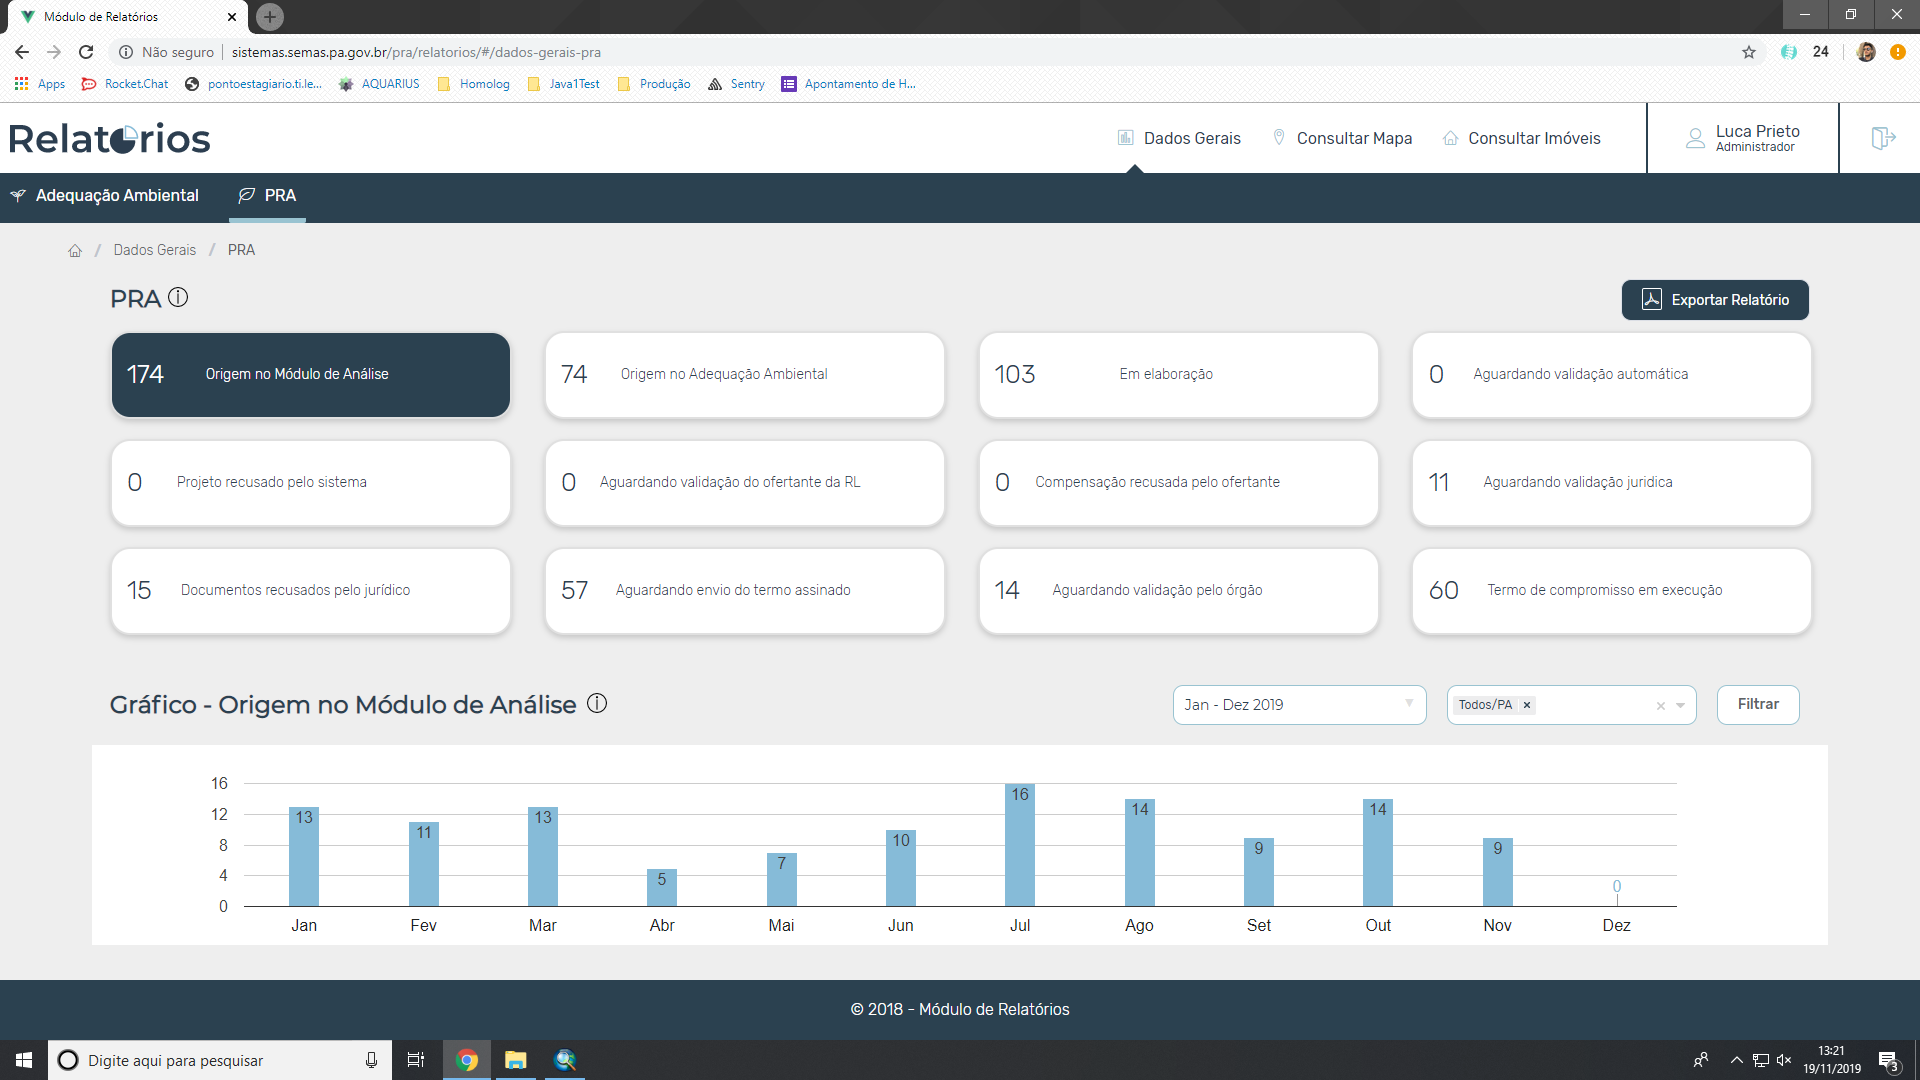
\includegraphics[scale=0.22]{relatorios-pra}\\  % o 0.9 indica 90% do tamanho original
% pdfLaTeX aceita figuras no formato PNG, JPG ou PDF
% figuras vetoriais podem ser exportadas para eps e depois convertidas para pdf usando epstopdf
{\small Fonte: http://sistemas.semas.pa.gov.br/pra/relatorios/#/dados-gerais-adequacao-ambiental} %Fonte da imagem
\label{fig:exemplo} %rotulo para refencia
\end{figure}

O projeto de relatórios foi o primeiro projeto que tive a honra de iniciar, com uma equipe formada de 4 pessoas (2 devs, uma tester e uma PO).
O projeto consistia em uma plataforma de relatórios sobre o Programa de regularização ambiental e Adequação ambiental.

A escolha da tecnologia foi deixada como escolha nossa, então pela ótima experiencias com VueJs e o alto desempenho do framework , escolhemos o mesmo para o frontend.
Porem pelo baixo conhecimento sobre backend, a escolha da tecnologia foi feita pelo outro Dev da equipe, que escolheu Spring Boot.
Como só tinha evoluído softwares e nunca começado um, houveram diversos gargalos no desenvolvimento, como criação de ambientes, scripts para automatização de deploy entre outros.

Porem apos 2 meses, fui transferido para uma equipe especial que não possuia tribo e que estava precisando de alguém com conhecimento em frontend e então me convocaram.
O projeto era uma POC(Prova de conceito) que uma empresa ligada a Agronomia havia comprado. Com prazos curtíssimos e complexidade alta, o projeto foi um dos mais difíceis que já havia trabalhado.
O projeto foi todo construído utilizando componentização, com o backend feito com uma arquitetura bem definida e documentada para que fosse possível evoluir sem dificuldade. Graças a esse começo bem estruturado o projeto ocorreu bem.

Após esse projeto, fui alocado na tribo Atlântida onde trabalhei juntamente com outro desenvolvedor em um projeto, o SEIRH-CMS.

\begin{figure}[H]
\centering
\caption{Seirh-CMS} %legenda
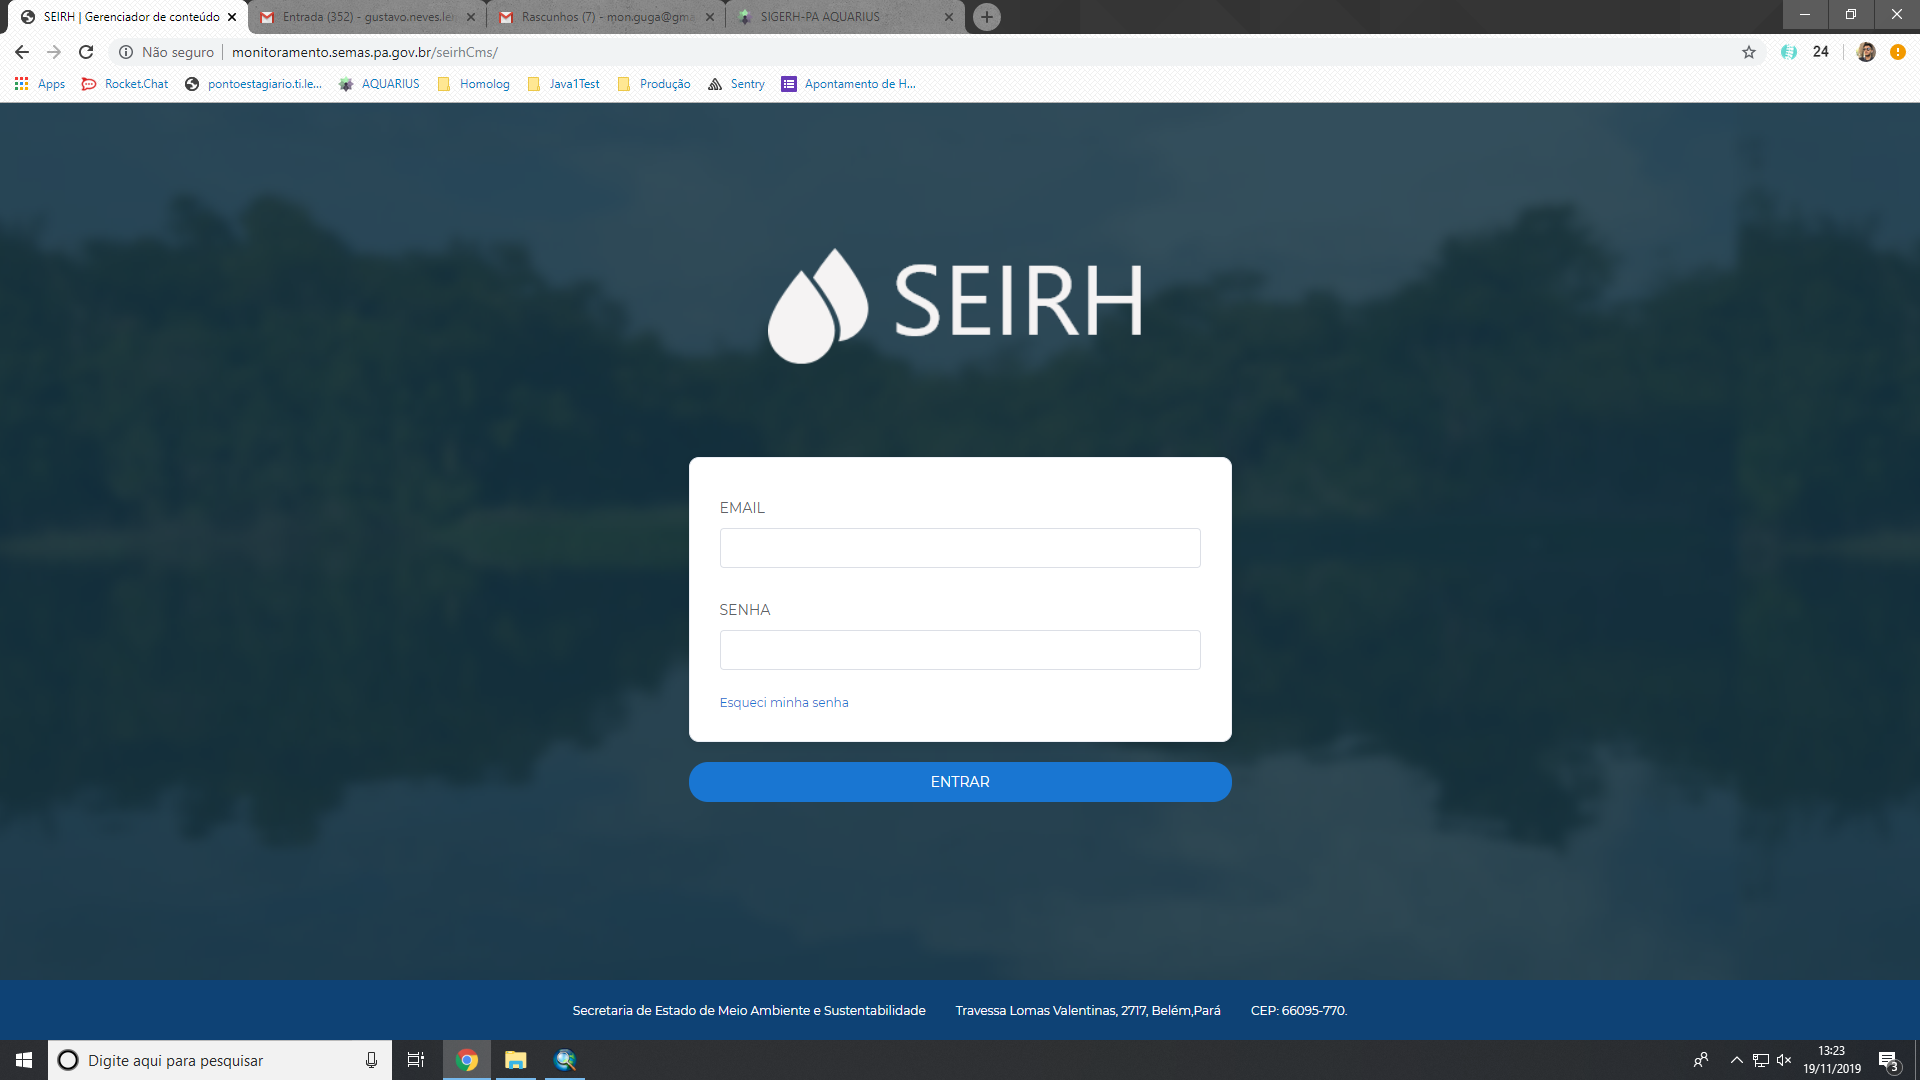
\includegraphics[scale=0.22]{seirh-cms}\\  % o 0.9 indica 90% do tamanho original
% pdfLaTeX aceita figuras no formato PNG, JPG ou PDF
% figuras vetoriais podem ser exportadas para eps e depois convertidas para pdf usando epstopdf
{\small Fonte: http://monitoramento.semas.pa.gov.br/seirhCms} %Fonte da imagem
\label{fig:exemplo} %rotulo para refencia
\end{figure}

O projeto do seirh-CMS era um gerenciador de conteúdo da aplicação seirh(Sistema Estadual de Informações Sobre Recursos Hídricos do Pará).
A plataforma web do seirh já existia, porem não havia comunicação com um backend, então seu conteúdo não era gerenciável, logo, havia a necessidade de uma refatoração total do sistema.

\begin{figure}[H]
\centering
\caption{Seirh} %legenda
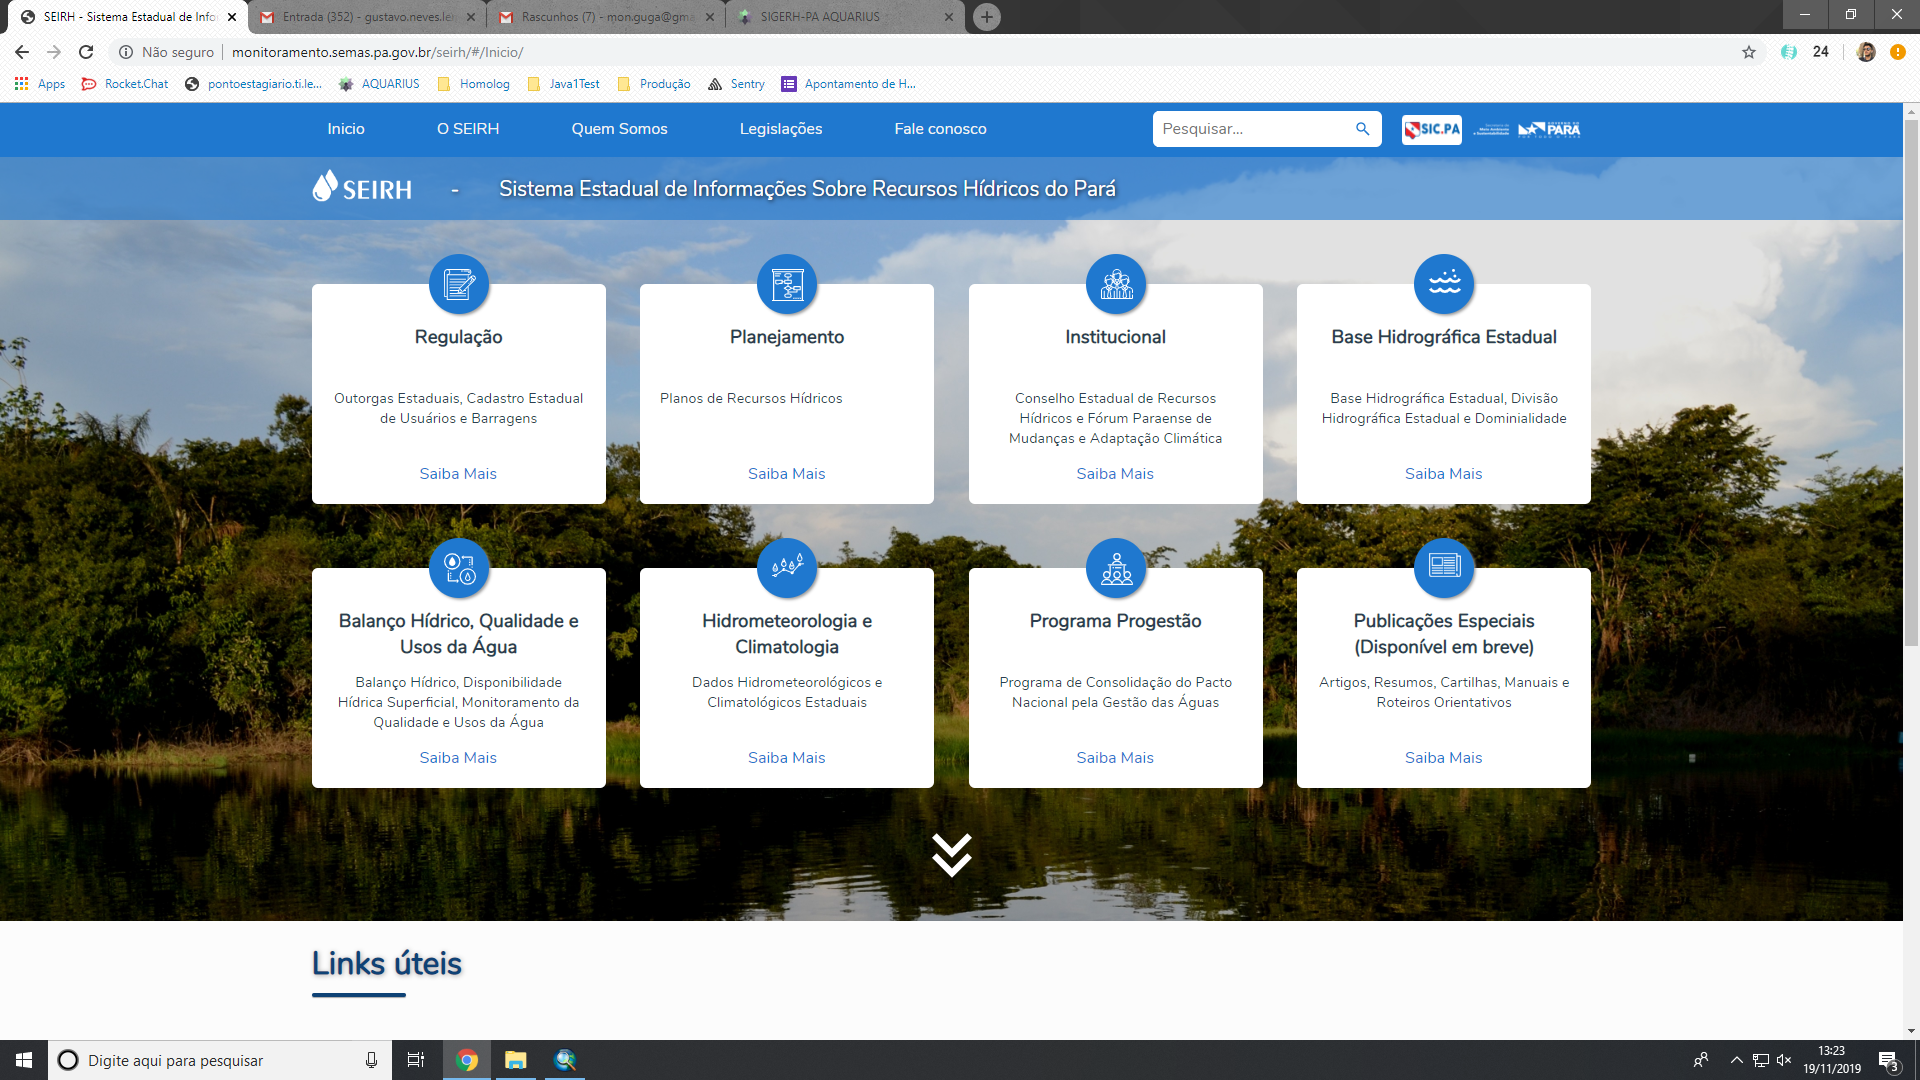
\includegraphics[scale=0.22]{seirh}\\  % o 0.9 indica 90% do tamanho original
% pdfLaTeX aceita figuras no formato PNG, JPG ou PDF
% figuras vetoriais podem ser exportadas para eps e depois convertidas para pdf usando epstopdf
{\small Fonte: http://monitoramento.semas.pa.gov.br/seirh} %Fonte da imagem
\label{fig:exemplo} %rotulo para refencia
\end{figure}

O prazo não diminui e então foi adicionado essa tarefa de refatoração ao nosso time.
Como já havia mais conhecimento sobre backend e toda tribo Atlântida ser constituída de desenvolvedores DotNet, resolvemos utilizar o framework DotNet Core 2.0, que 
provia diversas funcionalidades e atendia as nossas expectativas e necessidades.
Já o frontend continuou sendo feito com VueJs, uma vez que acabávamos de sair de projetos feitos com VueJs.

O projeto tinha como prazo 2 sprints(1 mes), um tempo muito curto e como era necessária a entrega, optamos por utilizar um quadro kanbam.
Foi minha primeira experiencia tomando liderança em prioridades das atividades, definição das atividades e organização no geral.

O projeto foi finalizado com excelência no prazo estipulado e graças a isso, fui realocado em um time que já trabalhava com DotNet e precisava de mais um desenvolvedor.

O projeto desta vez fazia parte de um grande complexo de plataformas que havia sido encomendado por uma empresa de agronomia e tinha muitos componentes de frontend parecidos.

Dai surgiu a iniciativa por parte minha e de outro desenvolvedor, de iniciar a construção do Design System da empresa.
Dai surgiu o Cria Design System, que é uma biblioteca de componentes UI para ReactJs.

Todos componentes eram criados pelo design do projeto, definido comportamentos e animações e depois desenvolvido. Para a visualização dos componentes separadamente, utilizamos o StoryBook,
que cria e organiza o catalogo de componentes e então para que essa biblioteca fosse compartilhada por toda empresa e não surgissem vários bugs, foram implementados testes automatizados para todos componentes e com uma nessesidade de cobertura de no minimo 80\%.

\begin{figure}[H]
\centering
\caption{Cria Design System} %legenda
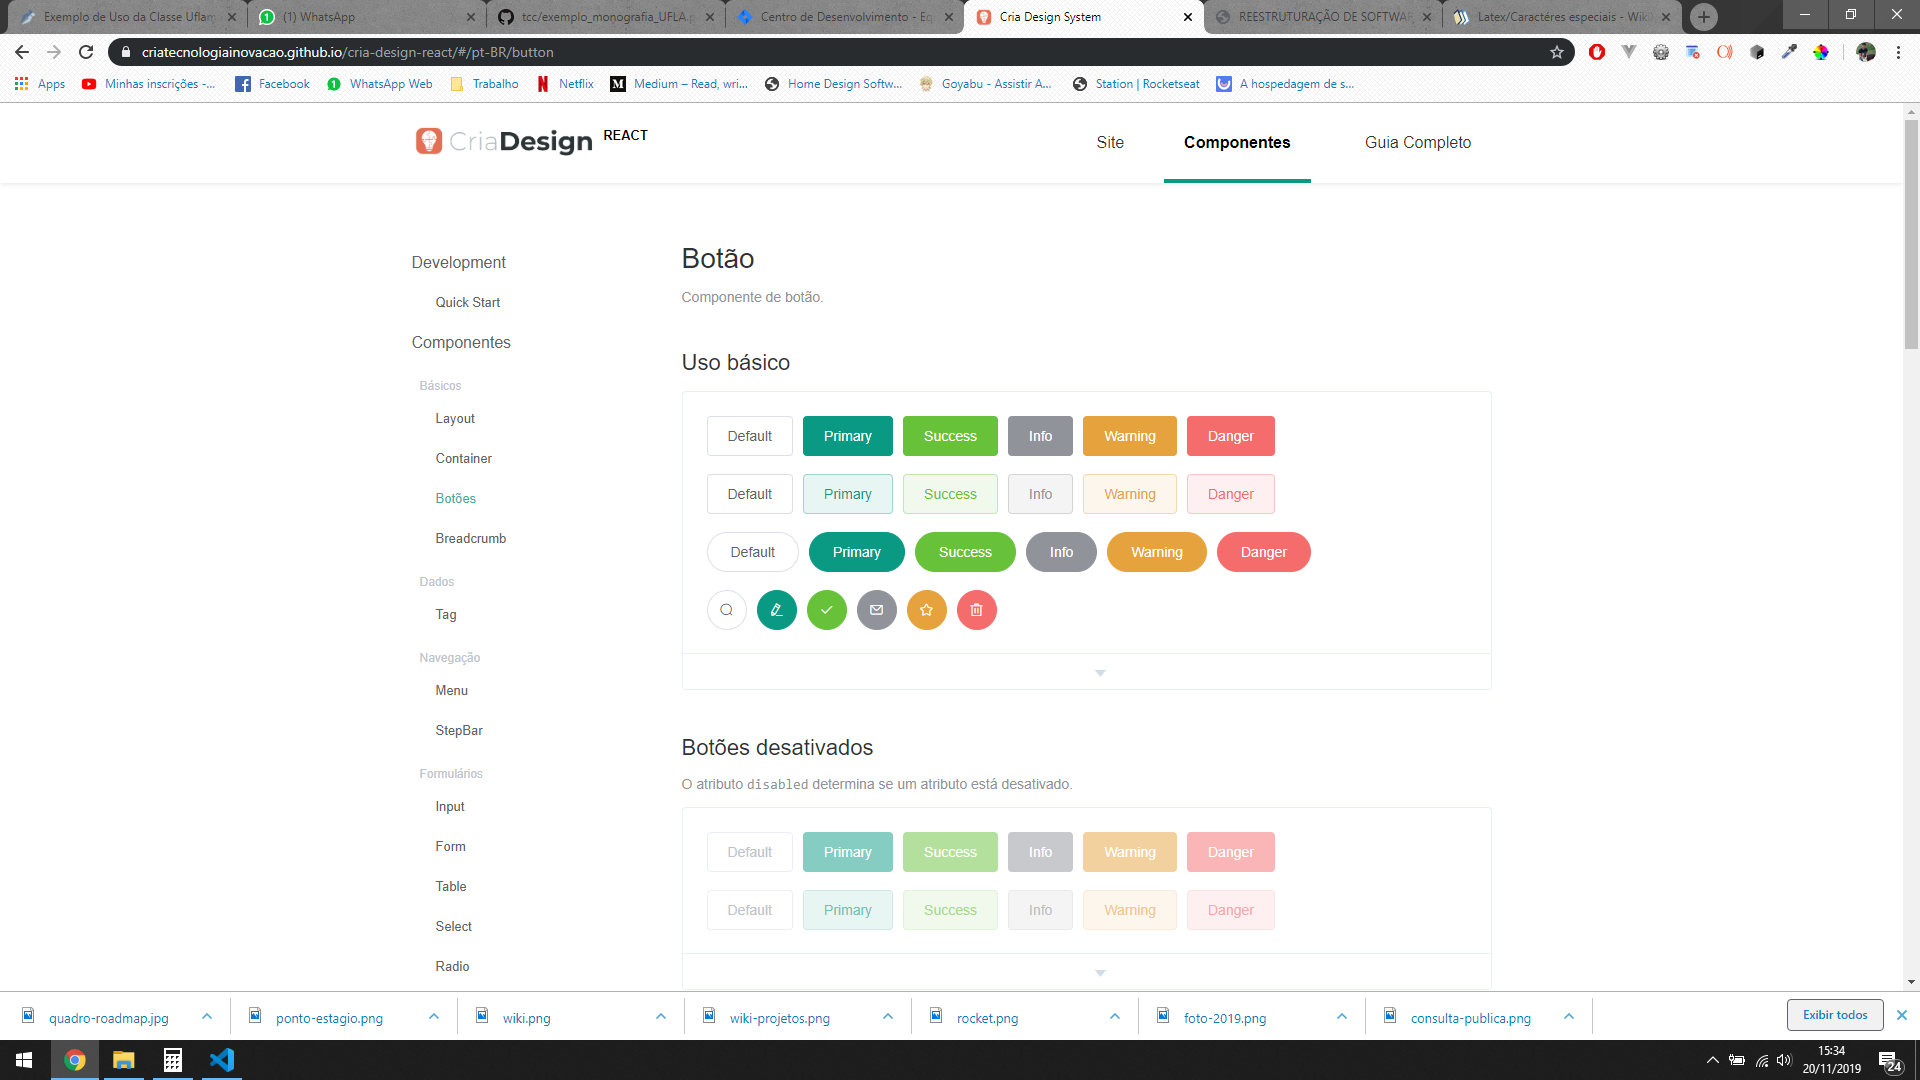
\includegraphics[scale=0.3]{cria-design}\\  % o 0.9 indica 90% do tamanho original
% pdfLaTeX aceita figuras no formato PNG, JPG ou PDF
% figuras vetoriais podem ser exportadas para eps e depois convertidas para pdf usando epstopdf
{\small Fonte: https://criatecnologiainovacao.github.io/cria-design-react/#/pt-BR/button} %Fonte da imagem
\label{fig:exemplo} %rotulo para refencia
\end{figure}

Apos ajudar com o começo do projeto e facilitar o desenvolvimento do mesmo, fui incorporado a uma equipe na mesma tribo e cuidava de alguns projetos como o SIOUT e Siger-pa.

\begin{figure}[H]
\centering
\caption{sigerpa} %legenda
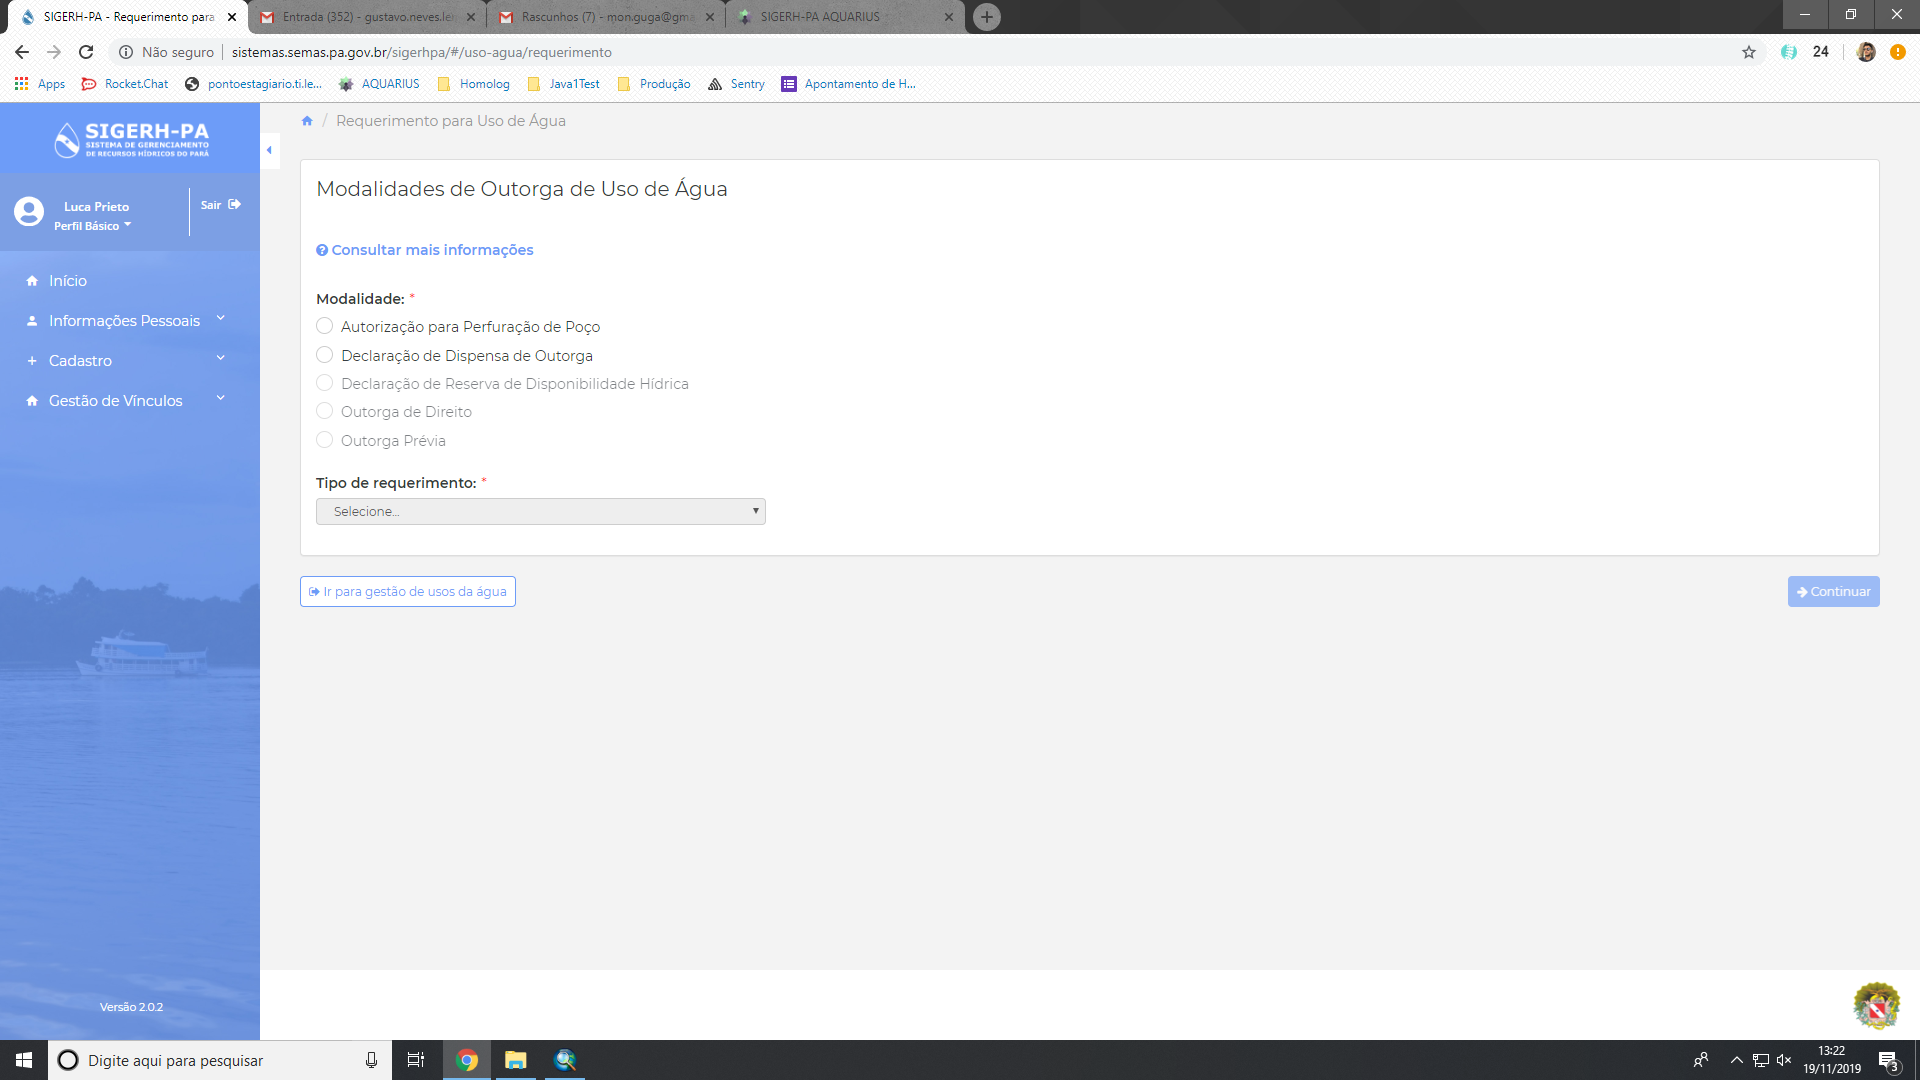
\includegraphics[scale=0.222]{sigerpa}\\  % o 0.9 indica 90% do tamanho original
% pdfLaTeX aceita figuras no formato PNG, JPG ou PDF
% figuras vetoriais podem ser exportadas para eps e depois convertidas para pdf usando epstopdf
{\small Fonte: http://sistemas.semas.pa.gov.br/sigerhpa/} %Fonte da imagem
\label{fig:exemplo} %rotulo para refencia
\end{figure}

O projeto do siger-pa(Sistema de Gerenciamento de Recursos Hídricos do Pará) é uma plataforma de cadastro e regularização de recursos hídricos(poços artesianos, nascentes e outros).
O projeto usava como backend o framework DotNet Framework 4.0 e como frontend AngularJs.

Até o fim do meu estágio, tive como tarefa evoluir e corrigir este sistema, que possuia vários problemas e alta complexidade por ser um sistema muito grande.
